% Source: https://tex.stackexchange.com/a/689270/6880

\documentclass[10pt,a4paper]{article}

\usepackage{amsmath,tikz}
\usetikzlibrary{positioning}
\begin{document}
    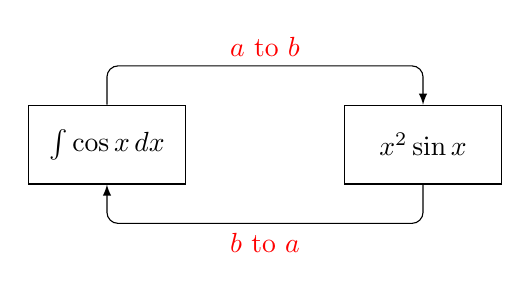
\begin{tikzpicture}
        \node[minimum width=2cm, minimum height=1cm, draw] (a) {$\int \cos x \,dx$};
        \node[minimum width=2cm, minimum height=1cm, draw, right=2cm of a] (b) {$x^2 \sin x$};
        \draw[-latex, rounded corners] (a) --++(90:1cm)-| node[near start, red, above]{$a$ to $b$} (b);
        \draw[-latex, rounded corners] (b) --++(-90:1cm) -| node[near start, red, below]{$b$ to $a$} (a);
    \end{tikzpicture}   
\end{document}